% Template para Proposta e TCC da EST/UEA -
% Padrão para os cursos do Núcleo de Computação
%
% Elaborado por Elloá B. Guedes
% Adaptado da versão elaborada por:				%                   Jucimar Maia Jr.
%
% Versão beta - 08 de outubro de 2015
%
\documentclass[a4paper,titlepage,12pt]{report}


\usepackage[utf8]{inputenc}
\usepackage[T1]{fontenc}
\usepackage{ae}
\usepackage[brazil]{babel}
\usepackage{a4wide}
\usepackage{comment}
\usepackage[pdftex]{graphicx,color}
\usepackage{graphics}
\usepackage{cite}
\usepackage{longtable}
\usepackage{float}
\usepackage{fancyvrb}
\usepackage{fancyhdr}
\usepackage{setspace}
\usepackage{amsmath}
\usepackage{lscape}
\usepackage{textcase}
\usepackage{anysize}
\usepackage{setspace}
\usepackage{booktabs}
\usepackage{url}
\usepackage{subfig}
\usepackage{cite}
\usepackage[alf]{abntex2cite}

\marginsize{20mm}{20mm}{20mm}{15mm}


%% Cabe�alhos
\renewcommand{\topfraction}{1}
\renewcommand{\bottomfraction}{1}
\renewcommand{\floatpagefraction}{1}
\renewcommand{\textfraction}{0}
%\renewcommand{\baselinestretch}{2}  
\doublespacing %espa�amento duplo
\sloppy

%% Nomes
\floatstyle{plain}  %%% tipos: plain, boxed, ruled
\newfloat{codigo}{tbp}{lop}[section]
\floatname{codigo}{C�digo}

%%% nome para ser usado no sum�rio

\newcommand{\listofcodename}{Lista de C\'{o}digos}



% RESUMO ----------------------------------------------------------------------------------------------------------------------------------------------------------------------

\newcommand{\resumo}[1]{
\begin{center} \LARGE \bf Resumo \end{center} 

\vskip 4em
\input{#1}

\newpage

}

% ABSTRACT ----------------------------------------------------------------------------------------------------------------------------------------------------------------------

\newcommand{\abstractt}[1]{
\begin{center} \LARGE \bf Abstract \end{center} 

\vskip 4em
\input{#1}

\newpage

}

% Sum�rio -----------
\newcommand{\sumario}{
\renewcommand{\contentsname}{Sum\'{a}rio}
\tableofcontents
\addcontentsline{toc}{chapter}{\listtablename}
\listoftables

\newpage
\addcontentsline{toc}{chapter}{\listfigurename}
\listoffigures
\addcontentsline{toc}{chapter}{\listofcodename}
\listof{codigo}{\listofcodename}  % Lista de C�digos

\clearpage
}



\pagestyle{plain}

\newcommand{\folhaRosto}[5]{

\thispagestyle{empty}
\begin{center}
\textbf{\\[0.4em]\MakeUppercase{#2} \\[5cm]}
\textbf{\MakeUppercase{#1}\\[96pt]}

\end{center}

\hspace*{8cm}
\begin{minipage}{8cm} 
Trabalho de Conclusão de Curso
apresentado à banca avaliadora do Curso de Engenharia de Computação, da 
Escola Superior de Tecnologia, da Universidade do Estado do Amazonas, como
pré-requisito para obtenção do título de Engenheiro de Computação.\\[40pt] 
\end{minipage} 

\begin{center}
Orientador(a): #3 \\[12ex]
Manaus -- #4 -- #5\\
\end{center}


\pagenumbering{roman}
\newpage
}



%% Preencha aqui os seguintes dados
\def \titulo{Uma Plataforma Web para Gerenciamento de Dados e Geração de Boletins Meteorológicos do LabInstru}
\def \orientador{Profa. Dra. Elloá Barreto Guedes da Costa}
\def \nome{Pedro Augusto Franco Ribeiro}
\def \mes{Novembro}
\def \ano{2017}

\begin{document}

\folhaRosto{\titulo}{\nome}{\orientador}{\mes}{\ano}

% Edite os seguintes arquivos para alterar as informações necessárias
% ficha Catalográfica------------------------------------------------------------------------------------------------------------------------------------------
\begin{spacing}{1.4}
\textit{\textbf{\\
Universidade do Estado do Amazonas - UEA\\
Escola Superior de Tecnologia - EST}}

\textit{\\
Reitor:\\ 
\textbf{
Carlos Eduardo de Souza Gonçalves}\\
Vice-Reitor:\\ \textbf{Nome do Vice-Reitor}}
\\
\textit{
Diretor da Escola Superior de Tecnologia:\\ 
\textbf{Mário Augusto Bessa de Figueirêdo}}
\\
\textit{
Coordenador do Curso de Engenharia de Computação:\\
\textbf{Antenor Ferreira Filho}}
\\
\textit{
Coordenador da Disciplina Projeto Final:\\
\textbf{Jucimar Maia da Silva Júnior}}
\\[12pt]
\textit{
Banca Avaliadora composta por: \hfill Data da Defesa:  /  /2015.\\
}
\textit{ 
\textbf{Profa. Dra. Elloá Barreto Guedes da Costa} (Orientador(a))\\
\textbf{Prof. M.Sc. }\\% Escreva o nome dos professor da sua banca antes de '\\' (comando para quebra de linha)
\textbf{Prof. M.Sc. }
}
\center{\bf CIP -- Catalogação na Publicação}\ \ \\
 \begin{small}
\begin{center}
\fbox{
\parbox{18cm}{
\begin{minipage}{17cm} 
L864a \hspace*{1cm} MARINHO, Deyvid Eric de Moraes\\[12pt]
\hspace*{2cm} \parbox{14cm}{
\hspace*{0.5cm}Desenvolvimento de Padrão para Monografias de Engenharia de Computação da UEA / 
Lanier Santos; [orientado por] Profa. Dra. Elloá Barreto Guedes da Costa -- Manaus: UEA, 2015.\\
\hspace*{0.5cm}240 p.: il.; 30cm\\
\hspace*{0.5cm}Inclui Bibliografia\\
\hspace*{0.5cm}Trabalho de Conclusão de Curso (Graduação em Engenharia de Computação).
Universidade do Estado do Amazonas, 2015.\\[6pt]
\hspace*{8cm} CDU: \hrulefill}
\end{minipage}}}
\end{center}
\end{small}
\end{spacing}
 \newpage

% folha de aprovação----------------------------------------------------------------------------------------------------------------------------------

\begin{center}
\bf \MakeUppercase{\nome}\\[1.5 cm]
\end{center}

\begin{center}
\bf \MakeUppercase{\titulo}\\[1.5cm]
\end{center}

\hspace*{8cm}
\begin{minipage}{8cm}

Trabalho de Conclusão de Curso apresentado à
banca avaliadora do Curso de Engenharia de Computação,
da Escola Superior de Tecnologia, da Universidade do Estado do Amazonas,
como pré-requisito para obtenção do título de
Engenheiro de Computação.\\

\large \bf Aprovado em: 05/12/2017
\end{minipage}

BANCA EXAMINADORA\\[12 pt]

\noindent \hrulefill \hspace*{6cm} \\
\noindent \textbf{\orientador}\\
\textit{UNIVERSIDADE DO ESTADO DO AMAZONAS}\\[0.5cm]

\noindent \hrulefill \hspace*{6cm} \\
\noindent \textbf{Profa. Márcia Sampaio Lima, M.Sc.}\\
\textit{UNIVERSIDADE DO ESTADO DO AMAZONAS}\\[0.5cm]

\noindent \hrulefill \hspace*{6cm} \\
\noindent \textbf{Prof. Flávio José Coelho, M.Sc.}\\
\textit{UNIVERSIDADE DO ESTADO DO AMAZONAS}\\



% Indique onde esta o arquivo do resumo
\resumo{./files/resumo.tex}
% Idem para o abstract
\abstractt{./files/abstract.tex}


\sumario

% Configuração de cabeçalhos
\pagestyle{fancy}
\renewcommand{\chaptermark}[1]{\markboth{#1}{}}
\renewcommand{\sectionmark}[1]{\markright{#1}}
\renewcommand{\headrulewidth}{0.5pt}
\newcommand{\rom}{\fontfamily{cmr}\fontseries{m}\fontsize{10}{12}\selectfont}
\fancyhf{} \fancyhead[LE,RO]{\rom\thepage}
\fancyhead[LO]{\rom\rightmark} \fancyhead[RE]{\rom\leftmark}
\fancypagestyle{plain}{
    \fancyhead{} % get rid of headers
    \renewcommand{\headrulewidth}{0pt} % and the line
 }


\pagenumbering{arabic} 


% Seus capítulos vão aqui --------
\chapter{Introdução}

As tecnologias computacionais relacionadas ao processamento de dados permitem uma melhor forma de manusear uma grande quantidade de informação. Se determinados processamentos fossem realizados manualmente, a quantidade de tempo necessária poderia inviabilizar a sua realização. Além disso, os eventuais resultados também poderiam estar sujeitos à erros de manipulação, os quais seriam difíceis de detectar. Considerado estas dificuldades, diversas áreas do cotidiano utilizam a tecnologia como uma aliada, por exemplo a Meteorologia, responsável pelo estudo do clima e das condições de tempo de uma determinada região.

Algumas das atribuições da Meteorologia compreendem o entendimento do estado presente da atmosfera, o chamado ``tempo meteorológico'', e a realização de previsões, a chamada ``previsão do tempo'' \cite{Vianello:Livro}. No caso do tempo meteorológico, se faz necessário medidas de diferentes variáveis como temperatura do ar, umidade relativa do ar, direção e velocidade do vento, precipitação, pressão atmosférica, radiação, dentre outras. Considerando o grande volume de dados comum a este domínio, é essencial que tecnologias, métodos e ferramentas auxiliem a realização dessas tarefas propostas.

Visando um melhor entendimento das questões meteorológicas de Manaus e da Amazônia, em março de 2010 foi fundado o \emph{Laboratório de Instrumentação Meteorológica} (LabInstru) da Escola Superior de Tecnologia (EST) da Universidade do Estado do Amazonas (UEA). Este laboratório dispõe, dentre outros, de uma estação meteorológica automática, localizada nas dependências da EST/UEA, sob as coordenadas \ang{03;05;32,5}S, \ang{60;00;59,69}W a 31 metros acima do nível do mar, na qual diversos sensores encontram-se instalados para medida e registros de diferentes variáveis meteorológicas \cite{Labinstru:EST}.

Além da manutenção da estação meteorológica, o LabInstru possui uma série de atribuições, tais como a organização dos dados coletados, disponibilização de dados para órgãos governamentais e para a sociedade, geração de boletins meteorológicos informativos, dentre outros. Atualmente, a maioria dessas atividades têm sido realizada de forma manual, um processo demorado e exaustivo, sujeito a erros e imprecisões e que requer mão de obra altamente especializada.

Para ilustrar o contexto considerado, um exemplo é apresentado na Figura \ref{fig:contexto}. Se um interessado desejar adquirir uma determinada informação, primeiramente deverá preencher um formulário online disponível no site do LabInstru e também entregar, presencialmente no próprio laboratório, o termo de compromisso adequado à sua solicitação devidamente preenchido (Etapa 1). Em seguida, a equipe do laboratório recebe uma notificação da solicitação (via e-mail) e inicia a preparação dos dados (Etapa 2). O passo seguinte consiste em consultar diferentes arquivos-texto resultantes da estação meteorológica a fim de precisar o intervalo de datas requerido (Etapa 3). A equipe irá agregar esses dados e utilizará aplicativos adequados para filtrar as variáveis meteorológicas requeridas pela solicitação (Etapa 4).

\begin{figure}[H]
	\centering
	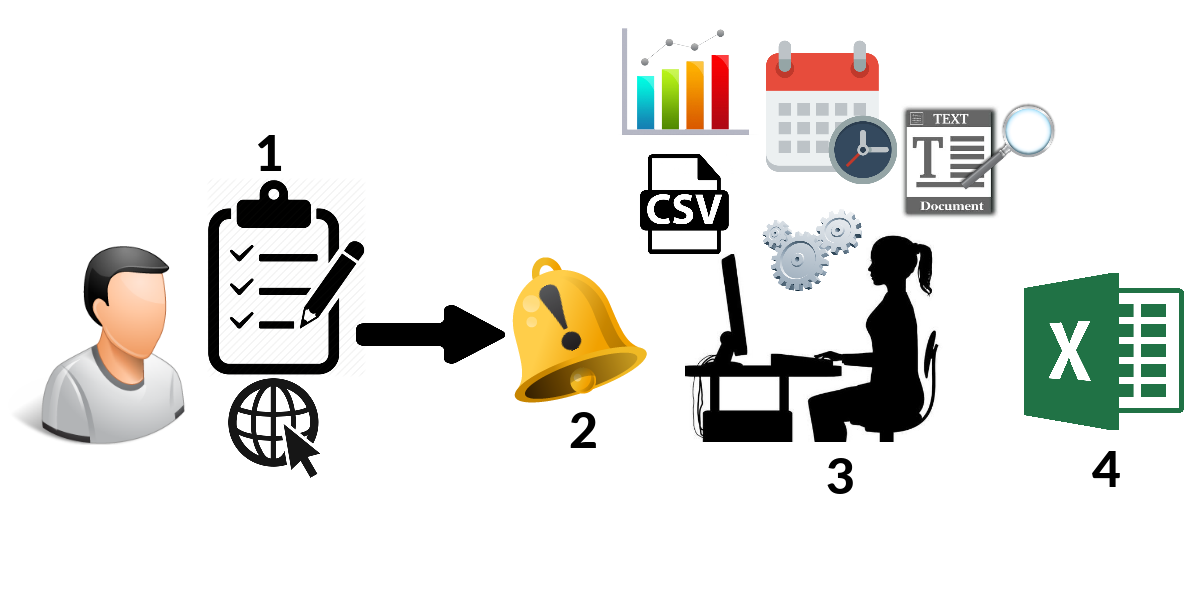
\includegraphics[width=0.6\textwidth]{./img/contexto.png}
	\caption{Contexto atual de uma das atividades realizadas pelo LabInstru. Fonte: Próprio Autor} 			\label{fig:contexto}
\end{figure}

Embora este exemplo ilustre o cenário atual do LabInstru, não compreende todas as dificuldades enfrentadas pela equipe do laboratório na realização de suas atribuições. Há que se mencionar as dificuldades na preparação de gráficos ilustrativos, na verificação da disponibilidade de dados, na geração de boletins meteorológicos, no controle e manuseio dos arquivos da estação meteorológica, dentre diversas outras.

Considerando este contexto, este trabalho de conclusão de curso teve por objetivo projetar e implementar uma plataforma web com vistas a colaborar na minimização das dificuldades mencionadas. Para tanto, contemplou o armazenamento, gerenciamento e disponibilização de dados da estação meteorológica automática da EST/UEA, administrada pelo LabInstru, fornecendo também uma visualização desses dados por meio de boletins meteorológicos.

\todo{Falta aqui uma visão geral sobre o que foi feito.}

\section{Objetivos}

O objetivo geral deste trabalho consistiu projetar e implementar uma plataforma web, para armazenamento, gerenciamento e disponibilização de dados de uma estação meteorológica automática. Para obtenção de sucesso no objetivo apresentado, fez-se necessário alcançar alguns objetivos específicos, a citar:

\begin{enumerate}
	\item Identificar e documentar as funcionalidades que a plataforma a ser desenvolvida deve prover;
	\item Elaborar protótipos de interface para validar as funcionalidades a serem desenvolvidas;
	\item Efetuar um levantamento das tecnologias para o desenvolvimento da plataforma web;
	\item Projetar e implementar a plataforma web;
	\item Implantar a plataforma web no LabInstru.
\end{enumerate}

\section{Justificativa}

O desenvolvimento de uma plataforma web para o LabInstru é importante por diversas razões. Primeiramente sabe-se que a forma como os dados meteorológicos são armazenados e as técnicas utilizadas para processamento influenciam diretamente na precisão e no tempo gasto para a realização de diversas tarefas. Assim, o desenvolvimento de uma plataforma para este domínio colabora diretamente na minimização destas dificuldades, visto que se propõe a  armazenar, gerenciar e disponibilizar os dados de maneira estruturada e automatizada.

Esta plataforma colabora de maneira direta com uma das atividades centrais do LabInstru, que compreende a organização dos dados coletados na estação instalada através do laboratório \cite{Labinstru:EST}. Há que se mencionar também que uma plataforma desta natureza favorece a divulgação dos dados meteorológicos produzidos. Estes são de interesse para pesquisadores de diversas áreas, para autoridades governamentais e também para a população em geral, como é amplamente visto na mídia.

Do ponto de vista da Engenharia de Computação, este trabalho de conclusão de curso também colabora com métodos e técnicas desta área do conhecimento aplicadas ao domínio da Meteorologia, auxiliando no desenvolvimento de uma plataforma que será usada em contexto real, por usuários reais e que irá colaborar para a manutenção de um laboratório de pesquisas de uma instituição pública de ensino superior, fomentando a realização de diversos outros trabalhos.

\section{Metodologia} \label{sec:metodologia}

A metodologia adotada para guiar as atividades deste trabalho de conclusão de curso é apresentada a seguir, a qual compreendeu a realização das seguintes atividades:

\begin{enumerate}[label=\textbf{Atividade \arabic*}.,leftmargin=*,labelindent=1em]
	\item Identificar um processo de desenvolvimento que possa acomodar as características do trabalho em questão, considerando que novos requisitos podem ser descobertos, que só há um desenvolvedor e que não deve haver \emph{overhead} na documentação das atividades;
	\item Estudo dos arquivos gerados pela estação meteorológica do LabInstru, pré-requisito para o entendimento de diversos requisitos;
	\item Efetuar a elicitação de requisitos funcionais e não funcionais referentes ao domínio do problema, construindo diagramas de caso de uso e documentando os requisitos descobertos apropriadamente;
	\item Utilizando uma ferramenta de \emph{mockups}, construir protótipos da interface gráfica que permitam validar junto ao cliente os requisitos identificados;
	\item Elencar uma ordem de implementação dos requisitos considerando as dependências entre os mesmos e o cronograma disponível do trabalho de conclusão de curso;
	\item Identificar tecnologias para o desenvolvimento da plataforma web, considerando \emph{frameworks} que possam ajudar nesta tarefa e também recursos que possam auxiliar no desenvolvimento do \emph{front-end}, permitindo a criação da interface gráfica com recursos que venham a prover uma boa usabilidade;
	\item Implementar os requisitos considerando a ordem anteriormente especificada;
	\item Escrever o trabalho de conclusão de curso I;
	\item Defesa do trabalho de conclusão de curso I;
	\item Implantar a plataforma web junto ao cliente, permitindo a utilização da mesma pelos pesquisadores do LabInstru. Avaliar a possibilidade de instalação em um servidor local ou hospedagem em um servidor externo;
	\item Escrever o trabalho de conclusão de curso II;
	\item Defesa do trabalho de conclusão de curso II.
\end{enumerate}

\section{Organização do Documento}

Para apresentar a solução proposta, este trabalho de conclusão de curso está organizado como segue. O Capítulo \ref{cap:fundamentacao} apresenta os conceitos essenciais que foram utilizados no desenvolvimento deste trabalho, incluindo o contexto da Estação Meteorológica da EST, o boletim meteorológico do LabInstru e conceitos da Meteorologia, tais como índice de calor e escala de Beaufort. O Capítulo \ref{cap:solucao} apresenta a solução proposta, contemplando desde uma visão geral da mesma, os artefatos de modelagem produzidos, protótipos e a versão executável da mesma implementada na linguagem de programação Python, com o \emph{framework} Web2py. Por fim, as considerações finais e sugestões de trabalhos futuros encontram-se descritos no Capítulo \ref{cap:consideracoes}.

\chapter{Fundamentação Teórica}
%\chapter{Exemplo}

\section{Tabela com o Pacote Booktabs}

Um exemplo de tabela com o pacote booktabs pode ser visto na Tabela \ref{tabela:exemplo}. A explica��o das tabelas sempre vem em cima e esse padr�o deve ser respeitado. A numera��o � autom�tica e a inser��o no �ndice tamb�m. Legal n�? \cite{Bennett:QuantumInformationSurvey}

Basta quebrar uma linha para criar um novo par�grafo. Neste par�grafo vou contar que tabelas no \LaTeX d�o um pouco de trabalho, mas nada que com paci�ncia n�o se resolva. Veja os links com dicas que coloquei nos coment�rios do arquivo \texttt{index.tex}.

\begin{table}[ht!]
\caption{Esta � uma tabela b�sica em \LaTeX com o pacote booktabs.} \label{tabela:exemplo}
\center{
\begin{tabular}{cccc}
\toprule
Parte 1 & Parte 2 & Parte 3 & Parte 4\\
\midrule
0,415 & 1,365 & 1,98 & 2,05\\
1,36  & 45,5  & 7,98 & 3,01\\
2,36  & 1,35  & 0,15 & 5,32\\
\bottomrule
\end{tabular}}
\end{table}



\section{Inser��o de Figuras}

Voc� pode inserir figuras JPG no \LaTeX! Veja o caso da Figura \ref{fig:exemplo}. Se voc� quiser outras configura��es e dicas, veja o seguinte endere�o: \url{http://en.wikibooks.org/wiki/LaTeX/Floats,_Figures_and_Captions}.

A explica��o da figura sempre vem embaixo da mesma. Isto aqui � um novo par�grafo apenas para ilustrar a id�ia geral de como escrever.

\begin{figure}[H]
\centering
\caption{Um exemplo de figura JPG inserida no \LaTeX.} \label{fig:exemplo}
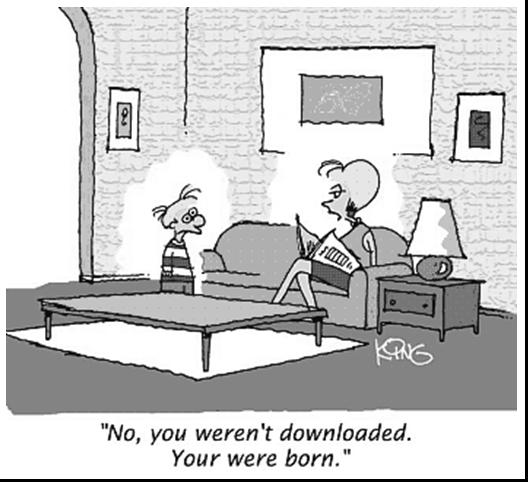
\includegraphics[width=0.4\textwidth]{./img/exemplo.jpg}\\
\small{Elaborado pelo autor.}
\end{figure}

Pode inserir v�rias figuras lado a lado tamb�m. Um exemplo est� reproduzido a seguir.

\begin{figure}[H]
  \centering
  \caption{Canal cl�ssico cuja obten��o da capacidade erro-zero � n�o-trivial.}
  \subfloat[\ ]{\label{fig:exG5}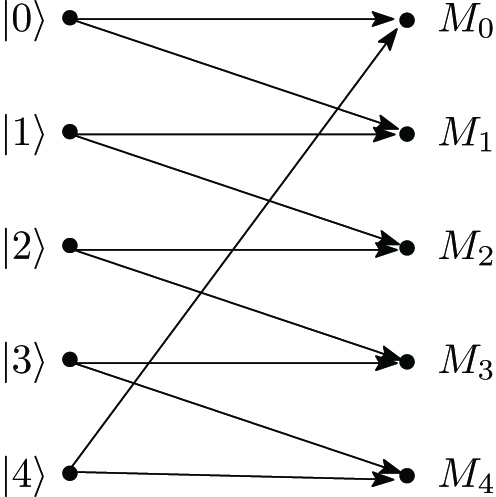
\includegraphics[width=0.3\textwidth]{./img/001}}
  \hspace{0.5cm}
  \subfloat[\ ]{\label{fig:exG52}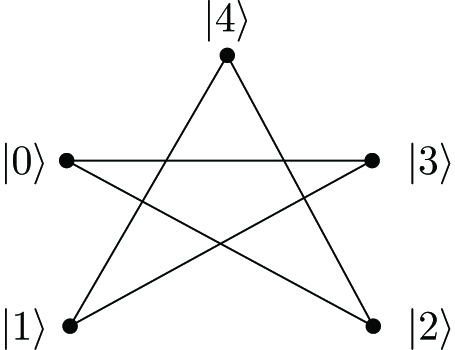
\includegraphics[width=0.3\textwidth]{./img/002}}
  \hspace{0.5cm}
  \subfloat[\ ]{\label{fig:exG53}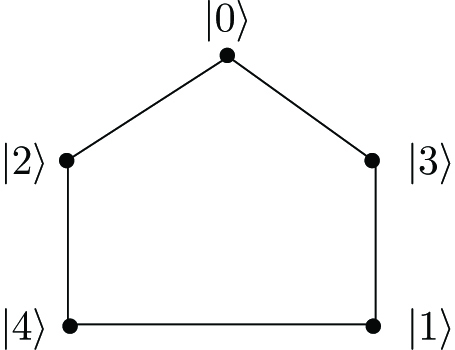
\includegraphics[width=0.3\textwidth]{./img/003}}\\
  \small{Elaborado por Bacon}
\end{figure}





\section{Refer�ncias Bibliogr�ficas no Padr�o ABNT}


%\chapter{T�tulo do Quarto Cap�tulo}


Vivamus ultricies tincidunt lacus ut pharetra. Sed fringilla hendrerit tempus. Suspendisse potenti. Cras hendrerit tortor ac est condimentum pellentesque. Morbi pretium lectus nec sapien laoreet eu malesuada diam adipiscing. Aliquam nisl ipsum, fermentum ut aliquam nec, varius sit amet nisi. Pellentesque interdum cursus malesuada. Vestibulum ante ipsum primis in faucibus orci luctus et ultrices posuere cubilia Curae; Nullam malesuada bibendum tortor, ut bibendum lorem varius eu. In eros orci, volutpat ut facilisis sit amet, commodo quis nulla.

Sed lectus metus, mollis nec vulputate id, imperdiet eget urna. Nam ut dolor at metus venenatis suscipit et in ligula. In hac habitasse platea dictumst. Mauris scelerisque dolor sed nisl mattis accumsan. Aliquam vulputate placerat feugiat. Pellentesque faucibus neque mi. Etiam porttitor varius tempus. Mauris varius porttitor posuere. Pellentesque iaculis imperdiet lobortis. Sed vulputate purus nec felis rutrum molestie.


\section{Algoritmos}




Nunc at fringilla dui. Pellentesque id tortor eu libero auctor rhoncus id vel velit. Duis auctor laoreet turpis, sed commodo tellus sollicitudin sit amet. Phasellus quis purus consectetur turpis hendrerit pretium eget in velit. Cras dignissim est vel mi malesuada a imperdiet velit condimentum. Vivamus ultrices diam non urna aliquet hendrerit. Sed lobortis, mauris quis egestas ullamcorper, nunc nulla auctor nulla, eu rutrum velit velit in nulla. Etiam lectus augue, pellentesque et porta at, pharetra id lectus. Duis eleifend eleifend mauris, nec mollis mauris vehicula nec. Nam sed ipsum ut massa lacinia vestibulum. Duis vitae sapien a lectus aliquam luctus eget sit amet nunc. Etiam a ipsum auctor tortor condimentum consectetur. Aliquam vestibulum libero sit amet nulla auctor aliquet. Sed laoreet imperdiet tellus non vulputate. Vivamus tristique ipsum vel metus venenatis in laoreet tortor hendrerit. Suspendisse potenti. Aenean tincidunt molestie libero sit amet porttitor. Class aptent taciti sociosqu ad litora torquent per conubia nostra, per inceptos himenaeos.





Cras nec quam mi, ut mattis ante. Lorem ipsum dolor sit amet, consectetur adipiscing elit. Sed fringilla auctor dictum. Nam hendrerit sapien sed massa consequat rutrum. Nullam congue, augue sed commodo malesuada, lectus nulla mollis magna, eget semper risus nisl eget elit. Duis vitae hendrerit massa. In a odio nunc, sit amet mollis dolor. In accumsan suscipit dui, a vestibulum diam condimentum ullamcorper. Etiam ut quam arcu, ac tristique ante. Vestibulum imperdiet elit non ante tristique accumsan. Donec vulputate fringilla tempor. Proin porttitor nisi nisi. Fusce vel ullamcorper orci. Lorem ipsum dolor sit amet, consectetur adipiscing elit. 

Vivamus ultricies tincidunt lacus ut pharetra. Sed fringilla hendrerit tempus. Suspendisse potenti. Cras hendrerit tortor ac est condimentum pellentesque. Morbi pretium lectus nec sapien laoreet eu malesuada diam adipiscing. Aliquam nisl ipsum, fermentum ut aliquam nec, varius sit amet nisi. Pellentesque interdum cursus malesuada. Vestibulum ante ipsum primis in faucibus orci luctus et ultrices posuere cubilia Curae; Nullam malesuada bibendum tortor, ut bibendum lorem varius eu. In eros orci, volutpat ut facilisis sit amet, commodo quis nulla.





% Referência segundo o padrão ABNT
% Edite este arquivo e inclua suas referências segundo a notação do Bibtex
\bibliography{ref}



\end{document}